%%%%%%%%%%%%
%
% $Autor: Wings $
% $Datum: 2019-03-05 08:03:15Z $
% $Pfad: SerialCommunication.tex $
% $Version: 4250 $
% !TeX spellcheck = en_GB/de_DE
% !TeX encoding = utf8
% !TeX root = filename 
% !TeX TXS-program:bibliography = txs:///biber
%
%%%%%%%%%%%%

\chapter{Serial Communication}


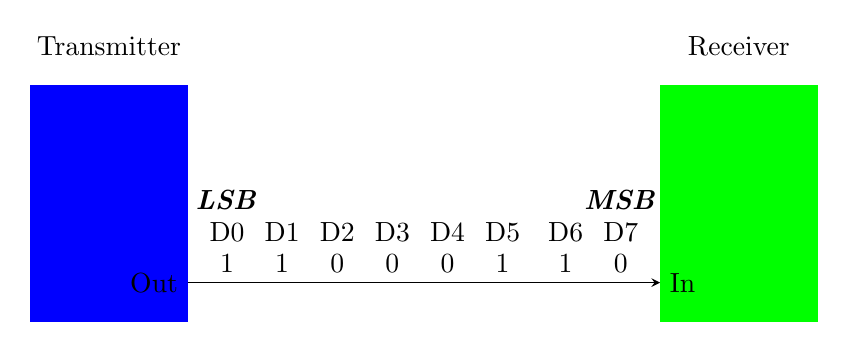
\begin{tikzpicture}

  % Left Rectangle (Blue)
  \draw[blue, fill=blue] (0,0) rectangle (2,3);
  \node[black] at (1,3.5) {Transmitter};

  % Right Rectangle (Green)
  \draw[green, fill=green] (8,0) rectangle (10,3);
  \node[black] at (9,3.5) {Receiver};

  % Connecting Line 
  \draw[->, >=stealth, fill=black] (2,0.5) node[left] {Out} --  (8,0.5) node[right] {In} ;

  % D0
  \node[above] at (2.5,0.5) {1};
  \node[above] at (2.5, 0.9) {D0};
  \node[above] at (2.5,1.3) {\textbf{\textit{LSB}}};
  
    % D1
  \node[above] at (3.2,0.5) {1};
  \node[above] at (3.2, 0.9) {D1};
  
    % D2
  \node[above] at (3.9,0.5) {0};
  \node[above] at (3.9, 0.9) {D2};
  
    % D3
  \node[above] at (4.6,0.5) {0};
  \node[above] at (4.6, 0.9) {D3};
  
    % D4
  \node[above] at (5.3,0.5) {0};
  \node[above] at (5.3, 0.9) {D4};
  
    % D5
  \node[above] at (6,0.5) {1};
  \node[above] at (6, 0.9) {D5};
  
    % D6
  \node[above] at (6.8,0.5) {1};
  \node[above] at (6.8, 0.9) {D6};
  
    % D7
  \node[above] at (7.5,0.5) {0};
  \node[above] at (7.5, 0.9) {D7};
  \node[above] at (7.5,1.3) {\textbf{\textit{MSB}}};
\end{tikzpicture}

\begin{center}
    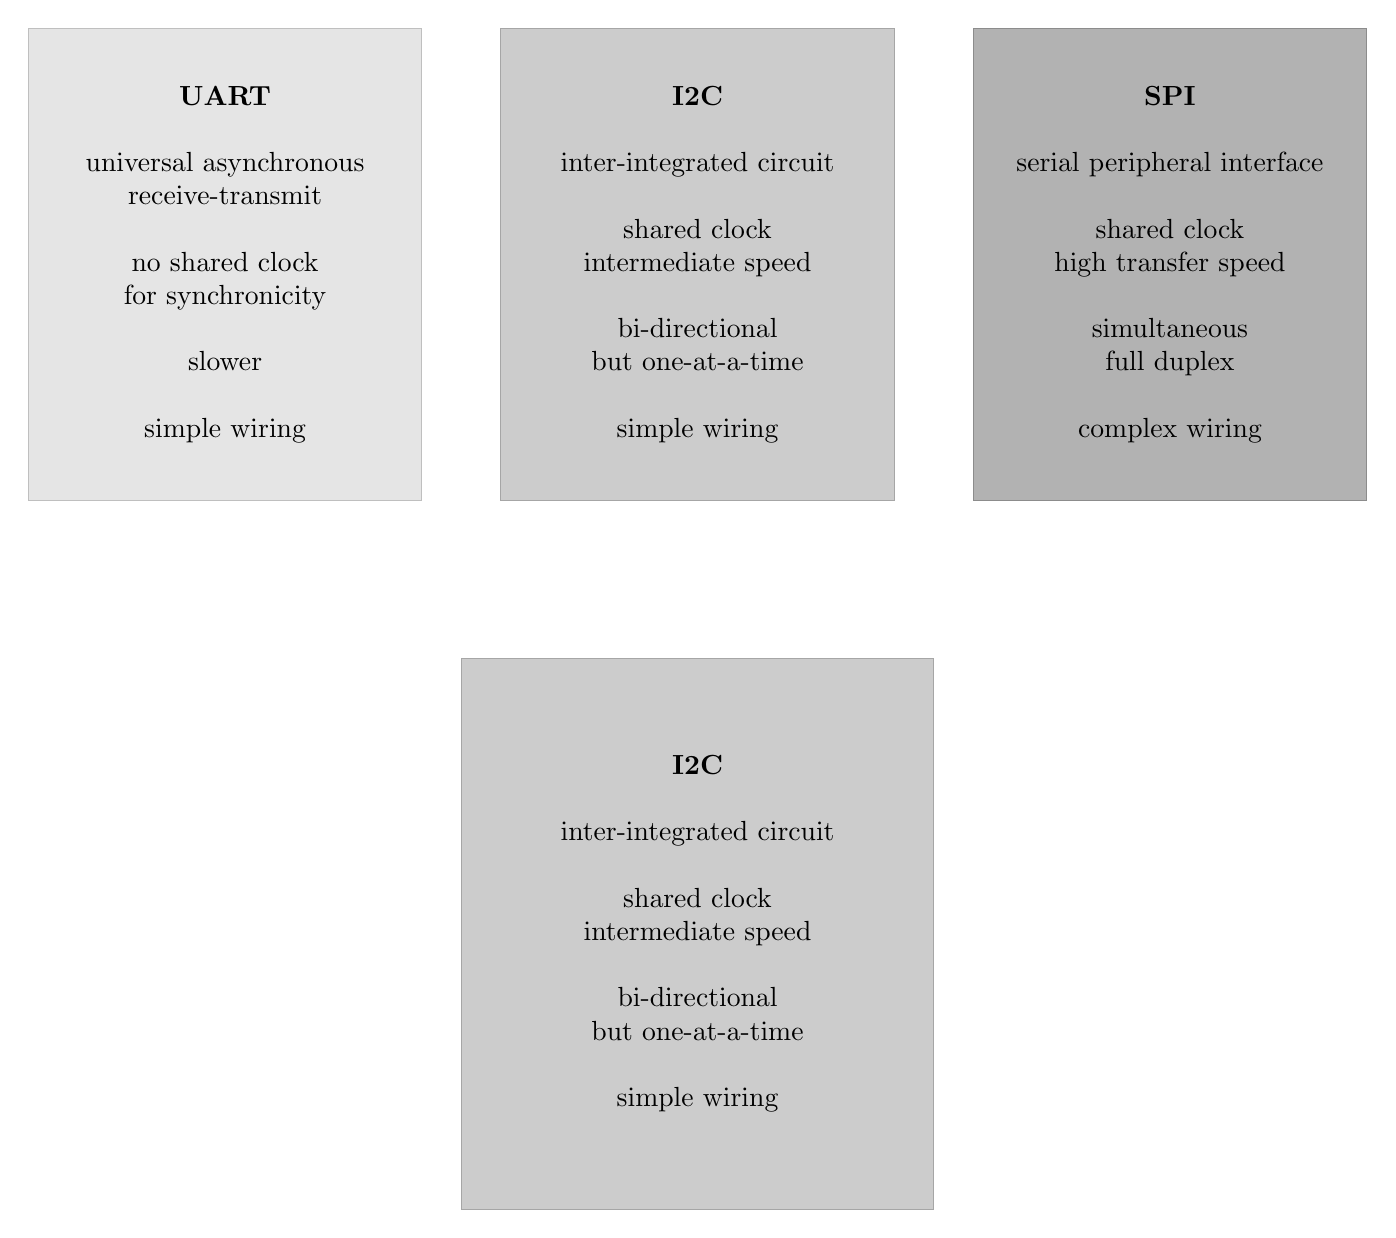
\begin{tikzpicture}
        % First Rectangle
        \draw[gray!50, fill=gray!20] (0,0) rectangle (5,6);
        \node[black, align=center] at (2.5,3) {%
            \textbf{UART} \\
            \\
            universal asynchronous \\
            receive-transmit \\
            \\
            no shared clock \\
            for synchronicity \\
            \\
            slower \\
            \\
            simple wiring
        };
        
        % Second Rectangle
        \draw[gray!70, fill=gray!40] (6,0) rectangle (11,6);
        \node[black, align=center] at (8.5,3) {%
            \textbf{I2C} \\
            \\
            inter-integrated circuit \\
            \\
            shared clock \\
            intermediate speed \\
            \\
            bi-directional \\
            but one-at-a-time \\
            \\
            simple wiring
        };
        
        % Third Rectangle
        \draw[gray!90, fill=gray!60] (12,0) rectangle (17,6);
        \node[black, align=center] at (14.5,3) {%
            \textbf{SPI} \\
            \\
            serial peripheral interface \\
            \\
            shared clock \\
            high transfer speed \\
            \\
            simultaneous \\
            full duplex \\
            \\
            complex wiring
        };
        
        % Additional Rectangle below the middle one
        \draw[gray!70, fill=gray!40] (5.5,-2) rectangle (11.5,-9);
        \node[black, align=center] at (8.5,-5.5) {%
            \textbf{I2C} \\
            \\
            inter-integrated circuit \\
            \\
            shared clock \\
            intermediate speed \\
            \\
            bi-directional \\
            but one-at-a-time \\
            \\
            simple wiring
        };
    \end{tikzpicture}
\end{center}